\documentclass[]{article}
\usepackage[T1]{fontenc}
\usepackage[utf8]{inputenc}
\usepackage[swedish]{babel}
\usepackage[margin=1.7in]{geometry}
\usepackage{mathtools}
\usepackage{graphicx}
\usepackage{listings}



%opening
\title{DD1350 Logik för dataloger \\ Laboration 2}
\author{Erik Ringdahl, erikrin@kth.se \\ Joel Tjärnstig, joelt@kth.se}

\begin{document}

\setlength\parindent{0pt}
\maketitle

\section{Verktygsutveckling}

\clearpage
\section{Modellering}
Vi valde att modellera en förenklad uttagsautomat. En användare möts först av en välkomstskärm. Användaren verifieras genom att ange sin pinkod. Om pinkoden är fel, bes användaren ange den igen. Om användaren anger rätt pinkod får ett belopp anges. Om beloppet inte kan tas ut får användaren skriva ett nytt belopp. Om beloppet finns tillgängligt tas pengarna ut och uttagsautomaten återgår till välkomstskärmen. Användaren kan även närsomhelst avbryta uttaget och återgå till välkomstskärmen.

\subsection{Tillståndsgraf}
Vi har 5 olika tillstånd (\textbf{Welcome Screen, Verify, Retry, Select Amount, Withdraw Money}) och 4 atomer (\texttt{Pin Entered, Failed, Verified, Valid Amount}).

\begin{figure}[h]
\centering
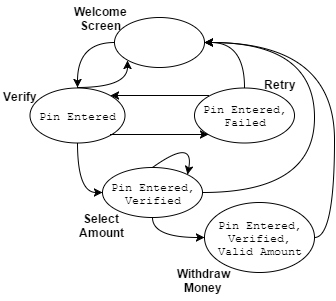
\includegraphics[width=0.75\linewidth]{modell}
\caption{Tillståndsgraf för uttagsautomat}
\label{fig:modell}
\end{figure}

\clearpage
\subsection{Prolog-kompatibel representation}
\begin{verbatim}
% States are ws(welcome screen), ve(verify), re(retry), 
% sa(select amount) and wm(withdraw money).
[
 [ws, [ve]],
 [ve, [ws, ve, re, sa]],
 [re, [ws, ve]],
 [sa, [ws, sa, wm]],
 [wm, [ws]]
].

% Labeling
[
 [ws, []],
 [ve, [pe]],
 [re, [pe, f]],
 [sa, [pe, v]],
 [wm, [pe, v, va]]
].
\end{verbatim}

\clearpage
\section{Specifiering}

\subsection{Hållbar systemegenskap}
Det finns en stig där så småningom det går att ta ut pengar.\\
\texttt{ef(and(and(pe,v),va))}

\subsection{Ohållbar systemegenskap}
Det finns en stig där något av nästa steg inte är välkomstskärmen.\\
\texttt{ef(not(ex(not(pe))))}

\section{Verifiering}
\subsection{Systemegenskaper}

\subsection{Tester}
Modellproveraren klarade alla tester.

\clearpage
\section*{Appendix}
\appendix

\section{Källkod}

%\lstinputlisting[language=Prolog]{logik.pl}



\end{document}